\documentclass{article}
\usepackage{graphicx}

\title{Devoir de Programmation : Tries}
\author{Marco PONTI\\ Nicolas SERRES}
\date{December 2016}

\begin{document}

\maketitle

\section{Introduction}

\paragraph{Question 1.1 : }

Le caractère pour le fin d'un mot est '@'

\paragraph{Question 4.10 :}

Calcule des complexitées PatriciaTrie :\\

findPrefix = O (longeur du mot)\\
(Parcours d'une chaine de caractère et comparaisons pour chaque caractère)\\

displayPtree = O (nb max de caractère * profondeur)\\
(Parcours d'une Hashmap au pire des cas contenant tout les caratères possible)
\\

cloneAll = O (nb max de caractère)\\
(Parcours d'une Hashmap au pire des cas contenant tout les caratères possible)
\\

search = O (4 * (longeur du mot))\\
(Une comparaison puis lancement de la sous fonction 4 comparaisons pour chaque
caractère du mot aux pire cas)\\

delete = O (4 * (longeur du mot))\\
(Une comparaison puis lancement de la sous fonction 4 comparaisons pour chaque 
caractère du mot aux pire cas)\\

insert = O ((5 * cloneAll) * longeur du mot)\\
(5 comparaison puis lancement de la fonction cloneAll, au pire cas pour chaque
caractères du mot)\\

countWord = O (nb max de caractère * profondeur)\\
(Une comparaisons et parcours d'une Hashmap au pire des cas contenant tout
les caratères possible pour toute la profondeur de l'arbre)\\

countDeep = O (nb max de caractère * profondeur)\\
(Une comparaisons et parcours d'une Hashmap au pire des cas contenant tout
les caratères possible pour toute la profondeur de l'arbre)\\

arrayWord = O (nb max de caractère * profondeur)\\
(Une comparaisons et parcours d'une Hashmap au pire des cas contenant tout
les caratères possible pour toute la profondeur de l'arbre)\\

allWord = O (nb max de caractère * profondeur)\\
(Une comparaisons et parcours d'une Hashmap au pire des cas contenant tout
les caratères possible pour toute la profondeur de l'arbre)\\

copy = O (nb max de caractère * profondeur)\\
(Parcours d'une Hashmap au pire des cas contenant tout les caratères
possible pour toute la profondeur de l'arbre)\\

split = O (cloneAll)\\
(Deux comparaisons et lancement de la fonction cloneAll)\\

fusion = O (2 * (nb max de caractère * profondeur-min-d'un-des-deux-arbres))
\\
(Deux comparaisons puis, parcours d'une Hashmap au pire des cas contenant
tout les caratères possible pour toute la profondeur de l'arbre le plus court)\\

getDeep = O (nb max de caractère * profondeur)\\
(Une comparaisons et parcours d'une Hashmap au pire des cas contenant tout
les caratères possible pour toute la profondeur de l'arbre le plus court)\\

mediumDeep = O (getDeep * profondeur)\\
(Appel getDeep puis Parcours la liste obtenu)\\

getPrefix = O (3 * longeur du mot)\\
(Trois comparaisons pour chaque caractère du mot)\\

convert = O ((nb caractère du préfix + nb max de caractère) * profondeur)\\
(Parcours du préfixe et parcours de la Hashmap des fils au pire des cas
contenant tout les caratères possible pour toute la profondeur de l'arbre)\\

Calcule des complexitées au pire Tries Hybrides : (nombre de comparaison)\\

ajouterMot = O (5 * (longeur du mot))\\

recherche = O (4 * (longeur du mot))\\

comptageMots = O (2 * nb de noeud)\\

listeMots = O 1 + (4 * nb de noeud))\\

comptageNil = O (nb de noeud)\\

hauteur = O (nb de noeud)\\

profondeurMoyenne = O (4 * nb de noeud)\\

prefixe = O ((4 * longeur du prefixe) + (2 * nb de noeud))\\

suppression = O (4 * (longeur du mot)) + (hauteur de l'arbre) + (4 *
longeur du mot * hauteur de l'arbre)\\

Conversion Hybrides vers Patricia = O ((4 * nb de noeud) + (nb de mot *
cloneAll * (longeur du mot)))\\

\newpage
\paragraph{Question 5.11 et 5.12 :}

Benchmark )\\

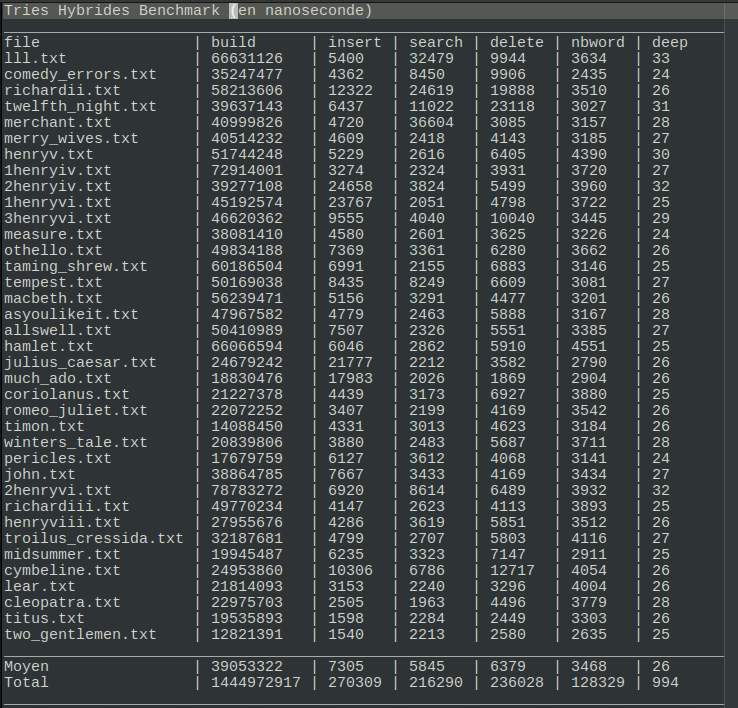
\includegraphics[scale=0.5]{BenchmarkPatc.png}

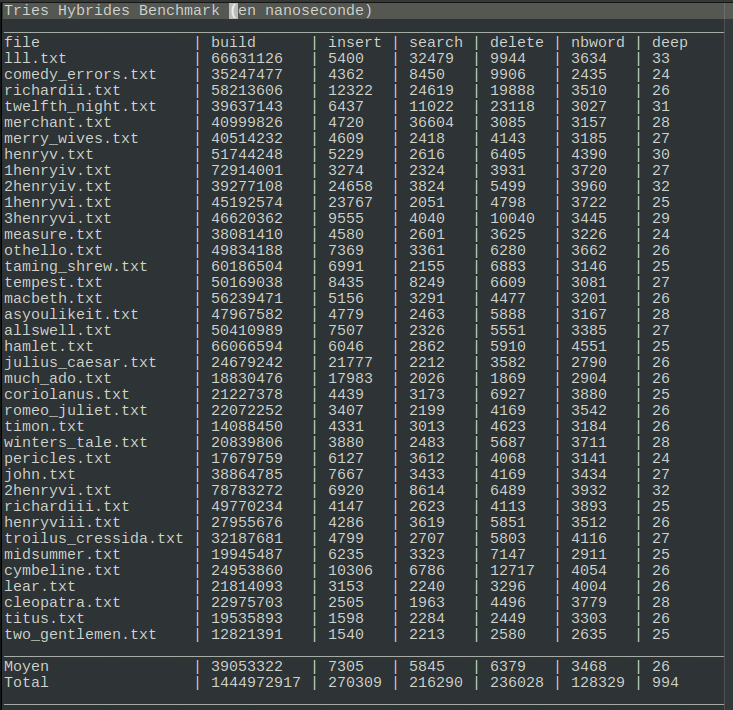
\includegraphics[scale=0.5]{BenchmarkHybc.png}

\paragraph{Conclusion :}

Sur quelque instance le Patricia-Tries est meilleur que le Hybride-Tries,
néanmoins, en moyen l'Hybride est moins performent en construction mais ensuite
il est plus rapide que le Patricia-Tries pour les fonctions d'insertion,
d'ajout, de suppression et de recherche

\end{document}